Microscopes are instruments designed to accomplish several important tasks to human knowledge, capable of magnifying images of small objects and structures which otherwise would not be seen by the human eye. It grants more information about the object of study to the research or the analysis. The first idea of the device was introduced by Romans, which discovered the magnifying property of glass in some sort of biconvex shape. Zacharias Janssen (1588-1632) was responsible for the invention of the first compound microscope with a concave eyepiece and  Francisco Fontana (1580-1656) introduced the convex eyepiece version of it \cite{zilio2009optica}. Furthermore, Robert Hooke (1635-1703) and Anton van Leeuwenhoek (1632-1723) were the most prominent science-related men responsible for microscope improvements \cite{wu2008microscope}. Due to the development of theories and their empirical proofs of veracity, in addition to the advances in hardware and software power, techniques such as image processing are applied to other fields. This also happens in microscopy, aiming to improve image quality, data reliability, and range of use \cite{boyde1990modern}.

This chapter provides information about bright-field and microscopy concepts in this work, describing the structure of the optical microscope, along with its uses and implications on the acquired images.

% Plenty of image degradation is due to the system acquisition process; in fact, defocus is a natural occurrence in optics, mainly caused by adjustments of the optical system.

% \subsection{Properties of the Spherical Lenses}
% Within the scope of this work, the main reason for introducing the concepts of optics is the imaging devices - the microscope, in particular. The structure of the apparatus will be described in Section \ref{sec:light_microscopy}. Moreover, a substantially large amount of devices rely on optical lenses for imaging, with properties such as depth of field and depth of focus.

As stated by \citeonline{halliday2013fundamentals}, \emph{lenses} are objects consisting of a transparent material, with a certain refractive index, that are made of two spherical surfaces on which light propagates and suffers refraction. They are used in optical systems due to their capacity to create images as long as their refractive index is not equal to that of the medium. Still, in agreement with \citeonline{halliday2013fundamentals}, some concepts related to lenses are important in our context and will be shown below. The following list depicts the principal elements from geometric optics that relates to lenses and its consequent imaging properties:

\begin{itemize}
    \item \emph{Radius of Curvature}: the distance between the center of the sphere and a refracting surface, named $\mathit{r_{1}}$ and $\mathit{r_{2}}$ on Figure \ref{fig:spherical_lens};
    
    \item \emph{Center of Curvature}: since the lenses are made by a union of two sections of a sphere-shaped object (which have a center), there are two Centers of Curvature for each lens, denoted by $\mathit{C_{1}}$ and $\mathit{C_{2}}$ on Figure \ref{fig:spherical_lens};
    
    \item \emph{Central Axis}: a line that represents the infinite number of radii of the sphere, which contain the center and the focal point;
    
    \item \emph{Focal Point}: also called \emph{focus}, a point within the central axis, where the image of the object is formed due to the convergence of the light rays from the object, and shown on Figure \ref{fig:spherical_lens} as $\mathit{F_{1}}$ and $\mathit{F_{2}}$;
    
    \item \emph{Focal Length}: presented as $\mathit{f}$ on Figure \ref{fig:spherical_lens}, it stands for the distance between the center of the sphere and the focal point;
    
    \item \emph{Object}: either a point or a surface on space that emits (or reflects) light and can be interpreted as a source;
    
    \item \emph{Image}: in this context, it is a representation of an object, formed by the action of lenses.
    
    \item \emph{Magnification}: a number that describes how larger or smaller the image will be in comparison to the object; mathematically, the ratio of the image distance to the object distance, both relative to the lens.
    
\end{itemize}

A single lens or a set of lenses (most of the optical systems are more complicated than a single lens) have the \emph{depth of field} and the \emph{depth of focus} properties. Although the terms appear to be similar, the former relates to objects and the latter, to images \cite{davidson2002optical}. For every system, there is a focal plane in which the formed images will be sharp. Depth of Field is the tolerance for the object focal plane that may produce sharp images, while Depth of Focus dictates the same tolerance for the image focal plane. In other words, depth of field is the zone in the real world that would yield an acceptably sharp image and depth of focus is the same idea for the imaging sensors or for plotting the image.Figure \ref{fig:spherical_lens} denotes an illustration of an arbitrary spherical lens.

\begin{figure}[htb]
	\centering
	\caption{\label{fig:spherical_lens} Arbitrary scheme of the optical properties of a spherical lens.}
	\begin{center}
	    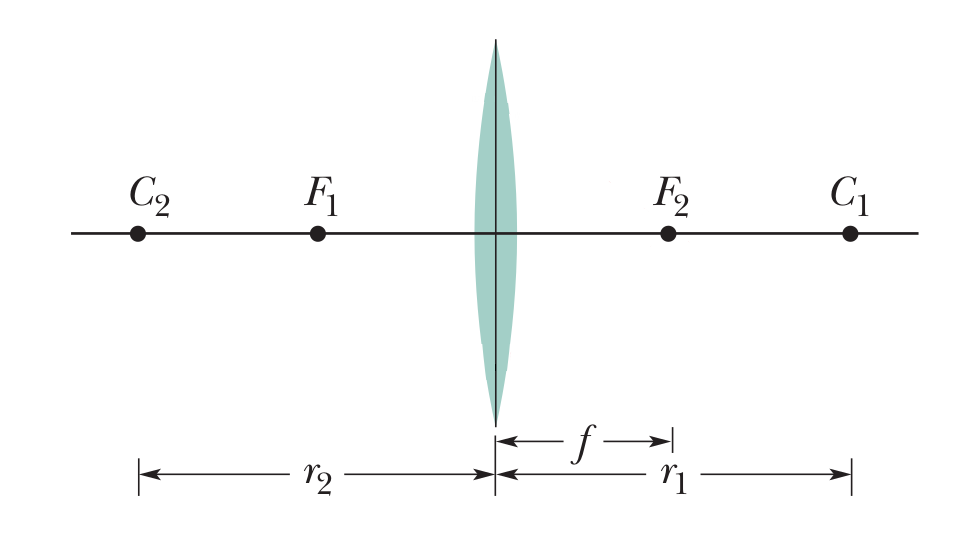
\includegraphics[scale=0.4]{images/fig4.png}
	\end{center}
	\centering
    \fadaptada{halliday2013fundamentals}
\end{figure}

Some properties of the spherical lenses directly influence the image formation process and, consequently, the resulting image quality. The \emph{numerical aperture}, as reported by \citeonline{murphy2012fundamentals}, is a measurement in terms of angles that shows how much lenses can capture light, and is given by

\begin{equation}
    \label{eqn:numerical_aperture}
    NA = n \sin{\theta},
\end{equation}

\noindent where $\theta$ is the half angle of the cone of specimen light accepted by the objective lens and $n$ is the refractive index between the lens and the specimen. There are optical flaws in lenses that hinder a proper image formation. Those are named \emph{aberrations} \cite{lawlor2019introduction}, and the most relevant types in the scope of this project are the \emph{spherical aberrations}. According to \citeonline{murphy2012fundamentals}, the spherical aberrations occur when there is a difference in the focal point of incident parallel rays at central and peripheral locations of a spherical lens' surface, which yields a blurred image of either a point source of light or an extended object. It is possible to correct a spherical aberration by changing the shape of the refracting surface, i.e. changing the radius of curvature for the lenses in order to adjust the focal point to one particular distance \cite{smith1988optics}. The illustration in Figure \ref{fig:spherical_aberrations} represents the spherical aberration for a point source of light, where it is possible to see the difference between incident rays in the borders and in the inner regions of the lens. The resulting image is, in this case, a set of concentric circles around a point.

\begin{figure}[htb]
	\centering
	\caption{\label{fig:spherical_aberrations} Arbitrary example of the spherical aberration.}
	\begin{center}
	    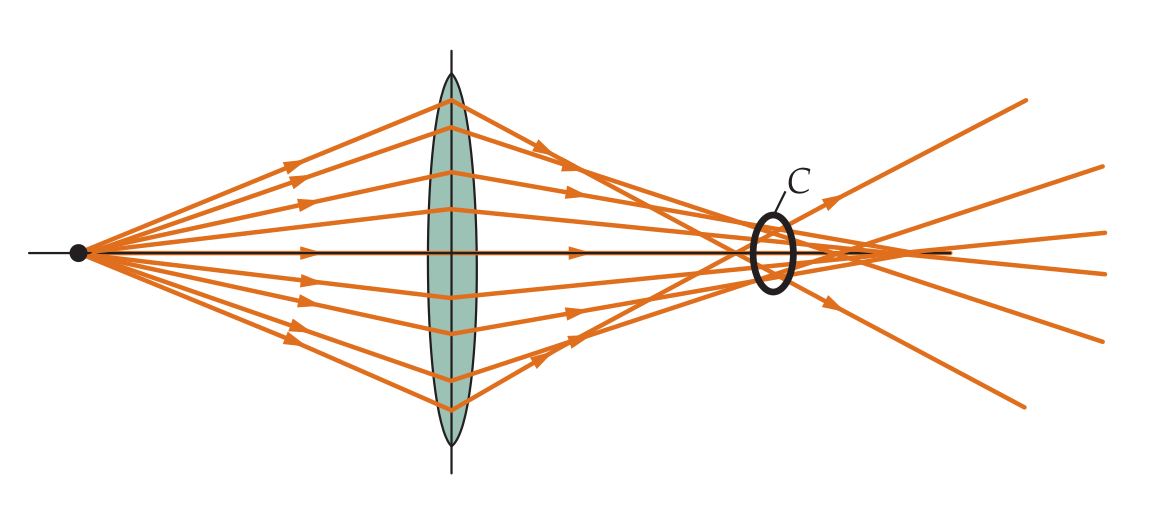
\includegraphics[scale=0.3]{images/spherical_aberration.png}
	\end{center}
	\centering
    \fdireta{tipler2008physics}
\end{figure}
    
\section{Light microscopy}
\label{sec:light_microscopy}

Historically, the structure of the first microscopes developed by Hooke and Leeuwenhoek had no eyepiece; the compound microscope, developed by Janssen, consists of the magnification lenses and also an eyepiece, which adds more magnification power and delivers the image to the user \cite{lawlor2019introduction}. As stated by \citeonline{murphy2012fundamentals}, the word \emph{compound} refers to the fact that the objective lens and the eyepiece (or ocular) work together to produce the final magnification of the image as a product of their magnifications. A graphical representation of the general structure of a compound microscope is shown in \autoref{fig:compound_microscope}, and as reported by \citeonline{bell2009introduction}, it consists of objective lenses, eyepieces, condensers, the stage and the light source.

\begin{figure}[H]
	\centering
	\caption{\label{fig:compound_microscope} Structure of the basic compound microscope: lenses that capture light rays from the specimen or object (objectives) or where the observer may look through (eyepieces), a collector of light from the light source (condenser), the support for the object (stage) and the light source.}
	\begin{center}
	    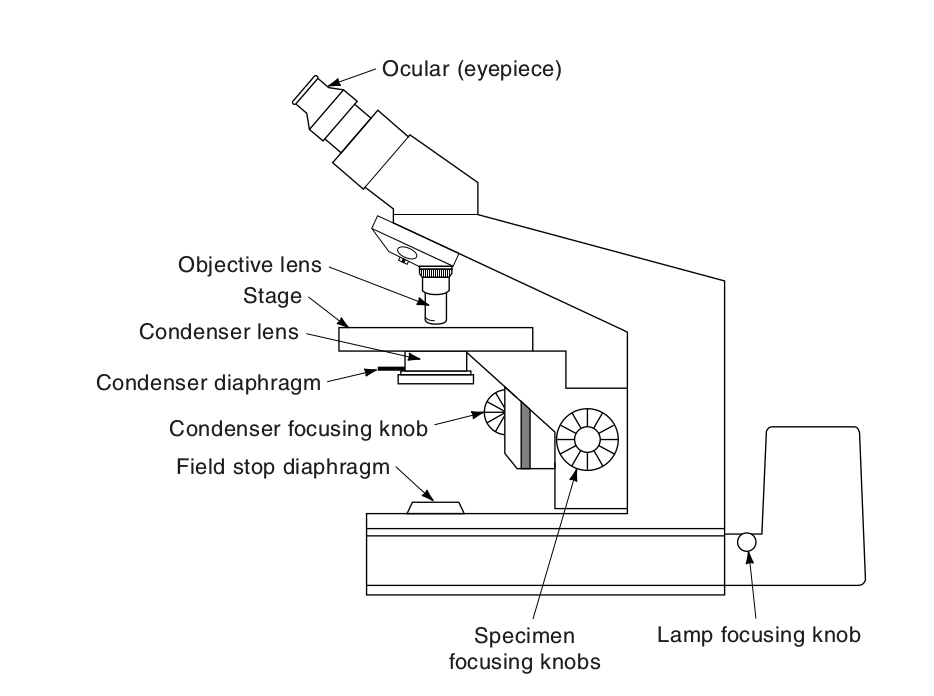
\includegraphics[scale=0.4]{images/fig5.png}
	\end{center}
	\centering
    \fdireta{bell2009introduction}
\end{figure}

Since light is some sort of radiation, there are several different ways to achieve imaging in microscopes; it can be made by light, polarized light, lasers, X-rays, among others. There are also advanced techniques such as confocal microscopy, which is capable of imaging a very small area of the object, with all the light rays focused on it \cite{rochow1994introduction}. The choice of the most suitable microscopy depends on the task.

According to \citeonline{dokland2006techniques}, the purpose of light microscopy is to provide magnified images of specimens by means of capturing emitted, reflected or transmitted light in the visible range of the spectrum, or even in the ultraviolet or near-infrared regions. As reported by \citeonline{lawlor2019introduction}, there are three general styles of light microscope. The \emph{upright microscope} is the easily affordable, easy to use traditional configuration with a light source on the base, a stage and the objective lenses. The \emph{inverted microscope} consists of the inverted configuration of an upright microscope, and offers some advantages when it comes to life sciences applications such as live cell imaging. Finally, the \emph{stereomicroscope} consists of a fusion of two compound microscopes in a convergent optical system and may have two different objectives and eyepieces or only one objective and two eyepieces \cite{schreier2004advances}. The former is named \emph{binobjective-binocular} (Greenough) and the latter \emph{monobjective-binocular}, or \sigla{CMO}{Common Main Objective Stereo Microscope}. One of the advantages of CMO microscopes is the higher depth of field, which allows the user to view and investigate biological specimens, relatively small materials and any kind of non-smooth surfaces. Furthermore, it is possible to view and acquire images in three dimensions \cite{rochow1994introduction}. The structure of both types of stereo compound microscopes is depicted in \autoref{fig:stereo_compound_microscope}.

\begin{figure}[htb]
	\centering
	\caption{\label{fig:stereo_compound_microscope} Graphic representation of the basic stereo compound light microscope structure, (a) for the Greenough type and (b) for the CMO.}
	\begin{center}
	    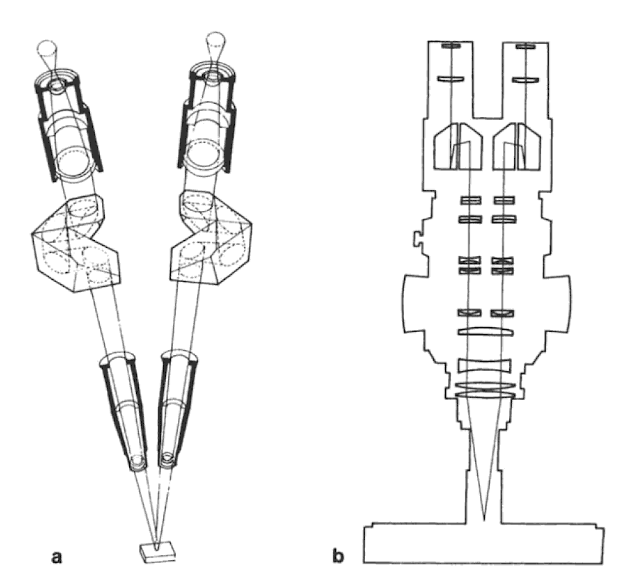
\includegraphics[scale=0.4]{images/stereomicroscope.png}
	\end{center}
	\centering
    \fdireta{rochow1994introduction}
\end{figure}

\subsection{Bright-field microscopy}
As for the use of light microscopes, there are several techniques and configurations which are achieved by varying the amount of lenses and light sources: bright-field, dark-field, phase-contrast, differential interference and fluorescence \cite{roane2009microscopic}. As stated by \citeonline{lawlor2019introduction}, images in bright-field microscopy are characterized by the contrast between the sample and the bright white background, generated by transmitted light. It is commonly used in pathology and histology fields for imaging fixed cells and tissues to reveal their structure, shape, and organization. The amount of light should be controlled, since the sample might suffer substantial changes, e.g. the chlorophyll molecules when illuminated by UV and visible light suffer irreversible breakdown (photodegradation) and generate other photoproducts \cite{petrovic2017clorophyll}. The \autoref{fig:bright-field_microscopy} provides an example of bright-field microscopy image.

\begin{figure}[htb]
	\centering
	\caption{\label{fig:bright-field_microscopy} Example of bright-field microscopy of a bone tissue.}
	\begin{center}
	    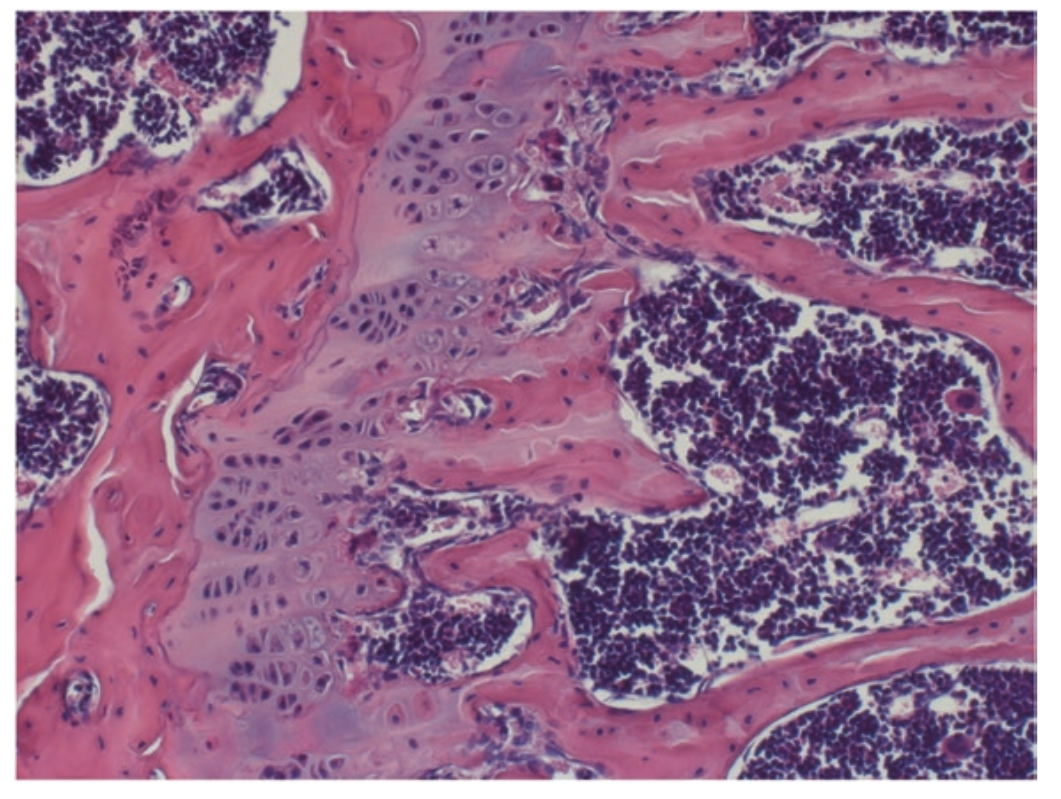
\includegraphics[scale=0.3]{images/bright-field_microscopy.png}
	\end{center}
	\centering
    \fdireta{lawlor2019introduction}
\end{figure}

The \textit{z-stacking} is a procedure to capture images in different positions concerning the $z$ axis, named slices, which may be applied to many different techniques to create a pseudo 3D image of the sample and consequently retrieve depth information about the specimen \cite{lawlor2019introduction}. The distance between each slice is dictated by the technique, either manually or automatically, and the focus needs to be adjusted at each slice. Next, the images must be aligned before any analysis is conducted. \autoref{fig:z-stack_example} represents a z-stacking example.

\begin{figure}[H]
	\centering
	\caption{\label{fig:z-stack_example} Z-stack images of yeast cells, acquired in positions under the focal plane (-15, -10 and -5 $\mu m$), exactly on it (0 $\mu m$) and above it (5, 10 and 15 $\mu m$).}
	\begin{center}
	    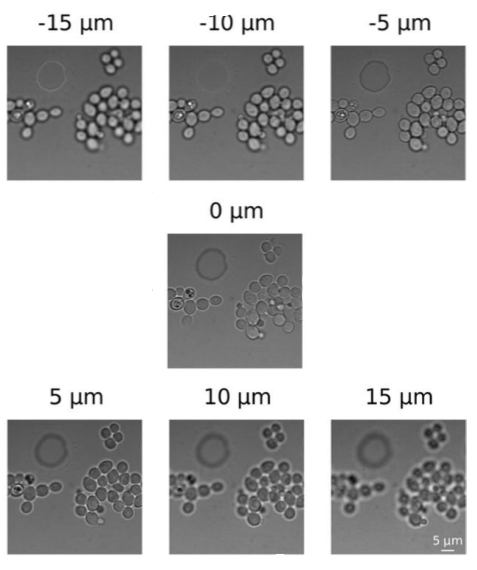
\includegraphics[scale=0.5]{images/z-stack.png}
	\end{center}
	\centering
    \fadaptada{wei2018neural}
\end{figure}